\begin{exercice*}
    \begin{enumerate}
        \item Construire, en rouge, l'image du triangle $ABC$ par la rotation de centre $R$ et d'angle \ang{90} dans le sens indiqué sur la figure.
        \item Construire, en vert, l'image du triangle $ABC$ par la rotation de centre $R$ et d'angle \ang{270} dans le sens indiqué sur la figure.
    \end{enumerate}
    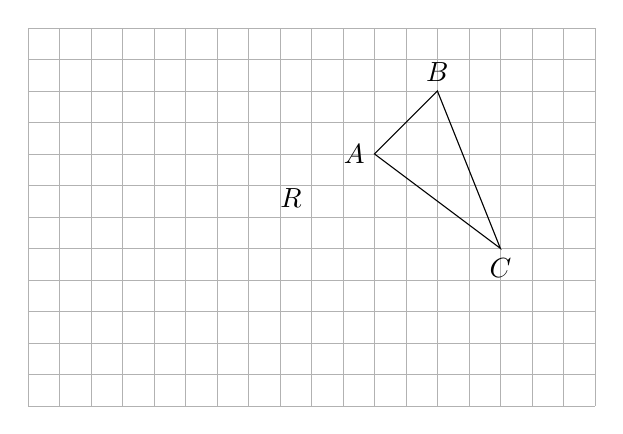
\begin{tikzpicture}[scale = 0.4]
        \draw[help lines, color=black!30] (0,0) grid (18,12);        
        \coordinate[label=above left:$R$] (R) at (9,6);
        \tkzDrawPoints[shape=cross out,size=3pt](R);
        \coordinate[label=left:$A$] (A) at (11,8);
        \coordinate[label=above:$B$] (B) at (13,10);
        \coordinate[label=below:$C$] (C) at (15,5);
        \draw (A)--(B)--(C)--cycle;
        \coordinate (O) at (15,9);
        \coordinate (M) at (17,9);
        \coordinate (N) at (15,11);
        \tkzDrawArc[thick,->](O,M)(N);
    \end{tikzpicture}
\end{exercice*}
\begin{corrige}
    %\setcounter{partie}{0} % Pour s'assurer que le compteur de \partie est à zéro dans les corrigés
    % \phantom{rrr}    
    \dots
\end{corrige}

